%\PassOptionsToPackage{svgnames}{xcolor}
\documentclass[oneside]{book}

\usepackage{geometry}

\usepackage{tcolorbox}
\usepackage{amsmath, amssymb, amsthm}
\usepackage{pdfpages}
\usepackage{sectsty}
\usepackage{multicol}
\usepackage{enumitem}
\usepackage{bm}
\usepackage{caption}
\usepackage{subcaption}
\usepackage{algpseudocode}
\usepackage{algorithm}
\usepackage{mathtools}

\chapterfont{\centering}

%\geometry{top=2cm, left=2cm, bottom=2cm, right=2cm}

%\usepackage{hyphenat}
%\hyphenation{ма-те-ма-ти-ка вос-ста-нав-ли-вать}
%\usepackage[utf8]{inputenc, vietnam}
\usepackage[T2A]{fontenc}
\usepackage[russian, vietnam]{babel}

\definecolor{green}{rgb}{0.0, 255.0, 0.0}
\definecolor{cyan}{rgb}{0.0, 255.0, 255.0}
\definecolor{red}{rgb}{255.0, 0.0, 0.0}
\definecolor{magenta}{rgb}{255.0, 0.0, 255.0}
\definecolor{yello}{rgb}{255.0, 255.0, 0.0}
\definecolor{white}{rgb}{255.0, 255.0, 255.0}

\geometry{a5paper}

\theoremstyle{definition}
\newtheorem{definition}{Định nghĩa}[chapter]
\newtheorem{theorem}{Định lý}[chapter]
\newtheorem{corollary}{Hệ quả}[chapter]
\newtheorem{lemma}{Bổ đề}[chapter]

\newtheorem*{remark}{Nhận xét}
\newtheorem*{axiom}{Tiên đề}
\newtheorem*{example}{Ví dụ}

\renewcommand*\contentsname{Mục lục}

\newcommand{\rank}{\text{rank}}
\newcommand{\RR}{\mathbb{R}}
\newcommand{\ZZ}{\mathbb{Z}}
\newcommand{\QQ}{\mathbb{Q}}
\newcommand{\lcm}{\text{lcm}}

\newenvironment{myexampleblock}[1]{%
    \tcolorbox[colback=LightGreen,colframe=DarkGreen,title=#1]}
    {\endtcolorbox}

\newenvironment{defblock}[2]{%
    \tcolorbox[colback=white,colframe=blue
    ,title=#1
    ]}
    {\endtcolorbox}

\newenvironment{theoremblock}[2]{%
    \tcolorbox[colback=white,colframe=magenta
    ,title=#1
    ]}
    {\endtcolorbox} 

\title{Nơi huyền thoại lưu danh}   
\author{Lê Quốc Dũng} 
\date{\today}

\begin{document}

%=========================================
\begin{titlepage}
		\centering{
			{\fontsize{40}{48}\selectfont 
			Nơi huyền thoại lưu danh}
		}\\
			
		\vspace{10mm}
		\centering{\Large{Lê Quốc Dũng}}\\
		\vspace{\fill}
		\centering \large{2023}
\end{titlepage}

\newpage
%\thispagestyle {empty}

\vspace*{2cm}

\begin{center}
	\Large{\parbox{10cm}{
		\begin{raggedright}
		{\Large 
			\textit{Đường đi ngàn dặm, bắt đầu bằng một bước chân.}
		}
	
		\vspace{.5cm}\hfill{Lão Tử}
		\end{raggedright}
	}
}
\end{center}

\newpage

\tableofcontents

\newpage

\textbf{Bảng các ký hiệu dùng trong sách}

\begin{table}[h]
    \begin{tabular}{c c}
        $\# S$ & số lượng phần tử của tập hợp $S$ (lực lượng của $S$)
    \end{tabular}
\end{table}

\newpage

\part{Đại cương toán học}
\chapter{Đại số cơ bản}

\section{Ánh xạ}

Cho 2 tập hợp $X$ và $Y$. Ánh xạ $f$ biến một phần tử $x \in X$ thành nhiều nhất một phần tử $y \in Y$.

Ta ký hiệu
\[f: X \rightarrow Y, \; f(x) = y\]

Khi đó, $X$ được gọi là tập nguồn (domain) và $Y$ là tập đích (image).

Ánh xạ có 3 loại:

\begin{itemize}[noitemsep]
    \item Đơn ánh (Injection): Hai phần tử khác nhau của tập nguồn cho hai ảnh khác nhau. Tức là với mọi $x_1, x_2 \in X$ mà $x_1 \neq x_2$, thì $f(x_1) \neq f(x_2)$
    \item Toàn ánh (Surjection): Mọi phần tử $y \in Y$ đều có ít nhất một phần tử $x \in X$ mà $f(x) = y$. Nói cách khác với mỗi phần tử trong $Y$ ta đều tìm được phần tử thuộc $X$ biến thành nó
    \item Song ánh (Injection): Nếu ánh xạ đó vừa là đơn ánh, vừa là toàn ánh
\end{itemize}

\begin{remark}
    Dựa vào định nghĩa và hình vẽ, ta có thể rút ra kết luận như sau
    \begin{itemize}[noitemsep]
        \item Đối với đơn ánh, do mọi phần tử của $X$ đều có ảnh ở $Y$, tuy nhiên có thể có phần tử ở $Y$ không do phần tử nào của $X$ biến thành (trong hình là 5). Do đó $| X | \leq | Y |$
        \item Đối với toàn ánh, mọi phần tử của $Y$ đều có nguồn gốc xuất xứ, tuy nhiên có thể có phần tử của $X$ không biến thành $y$ nào của $Y$ (trong hình là $e$). Do đó $| X | \geq | Y |$
        \item Đối với song ánh, do là kết hợp giữa đơn ánh và toàn ánh, khi đó dấu đẳng thức xảy ra, $| X | = | Y |$
    \end{itemize}
\end{remark}

\begin{figure}[ht]
    \centering
    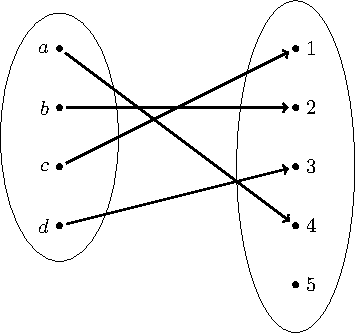
\includegraphics{pics/maps/injection.pdf}
    \caption{Đơn ánh}
\end{figure}

\begin{figure}[ht]
    \centering
    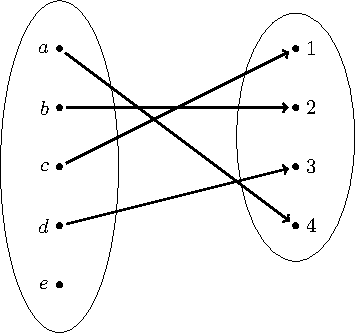
\includegraphics{pics/maps/surjection.pdf}
    \caption{Toàn ánh}
\end{figure}

\begin{figure}[ht]
    \centering
    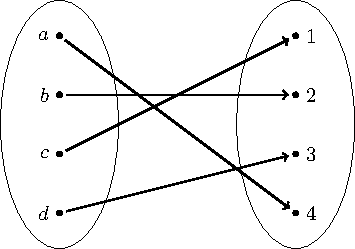
\includegraphics{pics/maps/bijection.pdf}
    \caption{Song ánh}
\end{figure}

\section{Hàm số}

Khi 2 tập nguồn và đích của ánh xạ là 2 tập hợp số, ta có hàm số.

\begin{example}
    Hàm số $f: \RR \rightarrow \RR$ với $y = f(x) = x^3 + x + 1$. Ở đây $X \equiv \RR$ và $Y \equiv \RR$.
\end{example}

Lưu ý rằng tập nguồn và đích không nhất thiết là tập hợp số cơ bản ($\QQ, \RR$) mà cũng có thể là tích Descartes của chúng.

\begin{example}
    Hàm số $f: \RR \times \RR \rightarrow \RR$ với $z = f(x, y) = x + y + xy$. Ở đây $X \equiv \RR$, $Y \equiv \RR$ và $Z \equiv \RR$.
\end{example}

Chúng ta còn một cách gọi khác cho đơn ánh, toàn ánh, song ánh trong tiếng Anh.

\begin{table}[ht]
    \centering
    \begin{tabular}{| l | l | l |}
        \hline
        đơn ánh & injection & one-to-one map \\
        \hline
        toàn ánh & surjection & onto map \\
        \hline
        song ánh & bijection & one-to-one and onto map \\
        \hline
    \end{tabular}

    \caption{Thuật ngữ tiếng Anh cho ánh xạ}
\end{table}
\chapter{Số học}

\section{Hàm Euler}

%\begin{defblock}{$\phi$ hàm Euler}
\begin{definition}[Phi hàm Euler]
    Cho số nguyên dương $n$. Số lượng các số dương nhỏ hơn $n$ và nguyên tố cùng nhau với $n$ được ký hiệu bởi $\phi(n)$ và gọi là $\phi$ hàm Euler. Nghĩa là
    \[\phi(n) = | \{ a : (a, n) = 1\} |\]
\end{definition}   
%\end{defblock}

Hàm Euler có ý nghĩa quan trọng trong lý thuyết số, công cụ giúp chúng ta giải các vấn đề về số mũ trong modulo.

Sau đây chúng ta xem xét hệ thặng dư đầy đủ và hệ thặng dư thu gọn.

Với số nguyên dương $n$, ta định nghĩa:

%\begin{defblock}{Hệ thặng dư đầy đủ}
\begin{definition}[Hệ thặng dư đầy đủ]
    Hệ thặng dư đầy đủ của $n$ là tập $\{0, 1, \ldots, n-1\}$.
\end{definition}
%\end{defblock}

Nói cách khác, hệ thặng dư đầy đủ của $n$ là các số dư có thể có khi chia một số bất kì cho $n$.

%\begin{defblock}{Hệ thặng dư thu gọn}

\begin{definition}[Hệ thặng dư thu gọn]
    Hệ thặng dư thu gọn của $n$ là tập các số $a$ mà $1 \leq a < n$ và $(a, n) = 1$. Số lượng các số $a$ như vậy là $\phi (n)$.  
\end{definition}

%\end{defblock}

\begin{remark}
    Hệ thặng dư thu gọn của $n$ gồm $\phi(n)$ phần tử là $$\{a_1, a_2, \ldots, a_{\phi(n)}\}$$
\end{remark}

\begin{remark}
    Nếu $n$ là số nguyên tố thì $\phi(n) = n-1$
\end{remark}

\section{Định lý Euler}

%\begin{theoremblock}{Định lý Euler}
    \begin{theorem}[Định lý Euler]    
        Cho số nguyên dương $n$. Với mọi số nguyên $a$ mà $(a, n) = 1$ thì 
        \[a^{\phi(n)} \equiv 1 \pmod n\]
    \end{theorem}
%\end{theoremblock}

\begin{proof}
    Giả sử $S = \{a_1, a_2, \ldots, a_{\phi(n)}\}$ là hệ thặng dư thu gọn của $n$. Ta sẽ chứng minh rằng nếu $a$ là số sao cho $(a, n)=1$ thì tập hợp
    $$\{a a_1, a a_2, \ldots, a a_{\phi(n)}\}$$ là hoán vị của tập $S$.

    Thật vậy, giả sử $a a_i \equiv a a_j \pmod n$ với $1 \leq i, j \leq \phi(n)$ và $i \neq j$.

    Do $(a, n) = 1$ nên tồn tại nghịch đảo $a' \pmod n$, nhân $a'$ cho 2 vế ta còn $a_i \equiv a_j \pmod n$.

    Nói cách khác, nếu $a_i \not\equiv a_j \pmod n$ thì $a a_i \not\equiv a a_j \pmod n$. Suy ra tập
    $$\{a a_1, a a_2, \ldots, a a_{\phi(n)}\}$$ là hoán vị của $S$.

    Ta nhân tất cả phần tử của $S$ thì sẽ bằng tích phần tử của tập trên
    $$a a_1 \cdot a a_2 \ldots a a_{\phi(n)} \equiv a_1 \cdot a_2 \ldots a_{\phi(n)} \pmod n$$

    Đặt $I = a_1 \cdot a_2 \ldots a_{\phi(n)}$ thì phương trình trên tương đương với 
    $$a^{\phi(n)} I \equiv I \pmod n$$
    
    Mà $(I, n) = 1$ do là tích các số nguyên tố cùng nhau với $n$ nên rút gọn 2 vế ta được
    $$a^{\phi(n)} \equiv 1 \pmod n$$

    Ta có điều phải chứng minh.
\end{proof}

\section{Định lý Fermat nhỏ}

%\begin{theoremblock}{Định lý Fermat nhỏ}
    \begin{theorem}[Định lý Fermat nhỏ]    
    Cho số nguyên tố $p$. Với mọi số nguyên $a$ thì $$a^p \equiv a \pmod p$$

    Khi $(a, p) = 1$ thì \[a^{p-1} \equiv 1 \pmod p\]
    \end{theorem}
%\end{theoremblock}

\begin{remark}
    Khi $(a, p) = 1$ thì định lý Fermat là hệ quả trực tiếp từ định lý Euler.
\end{remark}

\section{Tính chất hàm Euler}

\begin{remark}
    Với $(m, n) = 1$ thì $$\phi(m n) = \phi(m) \phi(n)$$
\end{remark}

\begin{proof}
    Ta viết các số từ 1 tới $mn$ thành bảng như sau

    \begin{center}
        \begin{tabular}{c c c c}
            1 & $m+1$ & $\cdots$ & $(n-1)m + 1$ \\
            2 & $m+2$ & $\cdots$ & $(n-1)m + 2$ \\
            $\cdots$ & $\cdots$ & $\cdots$ & $\cdots$ \\
            $m$ & $m+m$ & $\cdots$ & $(n-1)m + m$
        \end{tabular}
    \end{center}
    
    Hàng $r$ gồm các phần tử dạng $r m + k$ với $0 \leq r \leq n-1$ và $1 \leq k \leq m$. 
    Ta thấy rằng nếu $(rm + k, m) = 1$ thì $(k, m) = 1$.

    Do đó trên mỗi hàng có $\phi(m)$ phần tử nguyên tố cùng nhau với $m$.

    Tiếp theo, trên các hàng vừa tìm được, do $(m, n) = 1$ nên để $(rm + k, n) = 1$ thì $(r, n) = 1$.
    Nghĩa là có $\phi(n)$ hàng như vậy.

    Tổng kết lại, ta có $\phi(m) \phi(n)$ phần tử trong bảng nguyên tố cùng nhau với $mn$. Do đó có điều phải chứng minh.
\end{proof}
\chapter{Lý thuyết nhóm}

Câu chuyện bắt đầu vào một ngày khi mình vẫn còn sống ngày tháng tươi đẹp.

Cho tới khi học \textbf{lý thuyết nhóm} thì đời bớt đẹp hơn tí.

Để bắt đầu mình cần hiểu nhóm là gì.

\section{Nhóm}

%\begin{defblock}{Nhóm (Group)}
\begin{definition}{Nhóm (Group)}
    Một tập hợp $G$ và toán tử 2 ngôi $\star$ trên $G$ tạo thành một nhóm nếu:
    \begin{enumerate}[noitemsep]
        \item Tồn tại phần tử $e \in G$ sao cho với mọi $g \in G$ thì $g \star e = e \star g = g$. Khi đó $e$ được gọi là \textbf{phần tử đơn vị} của $G$.
        \item Với mọi $g \in G$, tồn tại $g' \in G$ sao cho $g \star g' = g' \star g = e$. Khi đó $g'$ được gọi là \textbf{phần tử nghịch đảo} của $g$.
        \item Tính kết hợp: với mọi $a, b, c \in G$ thì $a \star (b \star c) = (a \star b) \star c$.
    \end{enumerate}
\end{definition}

%\end{defblock}

%\begin{defblock}{Nhóm Abel}
\begin{definition}{Nhóm Abel}
    Nếu nhóm $G$ có thêm tính giao hoán, tức là với mọi $a, b \in G$ thì $a \star b = b \star a$ thì $G$ gọi là nhóm giao hoán hay nhóm Abel
\end{definition}
%\end{defblock}

Lý thuyết nhóm thuộc toán trừu tượng, và nó trừu tượng thật. Tuy nhiên khi học về nó mình dần hiểu hơn về cách toán học vận hành và phát triển.

\begin{example}
    Xét tập hợp số nguyên $\ZZ$ và phép cộng 2 số nguyên.
    \begin{enumerate}[noitemsep]
        \item Phần tử đơn vị là 0 vì với mọi $a \in \ZZ$ thì $a + 0 = 0 + a = a$
        \item Với mọi $a \in \ZZ$, phần tử nghịch đảo là $-a$ vì $a + (-a) = (-a) + a = 0$
        \item Phép cộng số nguyên có tính kết hợp do đó thỏa mãn điều kiện về tính kết hợp
    \end{enumerate}
    Như vậy $(\ZZ, +)$ tạo thành nhóm. Lưu ý do phép cộng 2 số nguyên có tính giao hoán nên đây cũng là nhóm Abel.
\end{example}

\begin{example}
    Xét tập hợp số hữu tỉ khác 0 $\QQ^*$ và phép nhân 2 số hữu tỉ. Ta thấy do $a, b \in \QQ^*$ nên tích $a \cdot b$ cũng khác 0, do đó cũng thuộc $\QQ^*$.
    \begin{enumerate}[noitemsep]
        \item Phần tử đơn vị là 1 vì với mọi $a \in \QQ^*$ thì $a \cdot 1 = 1 \cdot a = a$
        \item Với mọi $a \in \QQ^*$, phần tử nghịch đảo là $\frac{1}{a}$ vì $a \cdot \frac{1}{a} = \frac{1}{a} \cdot a = 1$
        \item Phép nhân 2 số hữu tỉ có tính giao hoán do đó thỏa mãn điều kiện về tính kết hợp
    \end{enumerate}
    Tương tự như nhóm $\mathbb{Z, +}$, nhóm $(\QQ^*, \cdot)$ cũng là nhóm Abel.
\end{example}

\section{Nhóm con}

\begin{definition}{Nhóm con (Subgroup)}
    Cho nhóm $(G, \star)$. Tập hợp $H \subset G$ được gọi là \textit{nhóm con} của $G$ nếu với mọi $a, b \in H$ thì $a \star b \in H$
\end{definition}
 
Nghĩa là toán tử $\star$ đóng với các phần tử trong $H$.

\begin{example}
    Xét nhóm $(\ZZ, +)$ như trên. Ta xét tập con gồm các số chẵn của nó
    \[2\ZZ = \{\ldots, -4, -2, 0, 2, 4, \ldots\}\]

    Ta thấy rằng tổng 2 số chẵn vẫn là số chẵn, nghĩa là phép cộng số nguyên đóng trên $2\ZZ$.
    Do đó $(2\ZZ, +)$ là nhóm con của $(\ZZ, +)$.

    Như vậy mọi tập hợp có dạng $n \ZZ$ đều là nhóm con của $(\ZZ, +)$.
\end{example}

\section{Coset}

\begin{definition}{Coset}
    (tạm dịch - \textit{lớp kề} theo wikipedia) Cho nhóm $G$ và nhóm con $H$ của $G$.

    Coset trái của $H$ đối với phần tử $g \in G$ là tập hợp
    \[gH = \{gh : h \in H \}\]

    Tương tự, coset phải là tập hợp
    \[Hg = \{hg : h \in H \}\]
\end{definition}

Từ đây nếu không nói gì thêm ta ngầm hiểu là coset trái.

Ví dụ với nhóm con $2\ZZ$ của $\ZZ$, ta thấy rằng

\begin{enumerate}
    \item Nếu $g \in \ZZ$ là lẻ thì khi cộng với bất kì phần tử nào của $2\ZZ$ ta có số lẻ
    \item Nếu $g \in \ZZ$ là chẵn thì khi cộng với bất kì phần tử nào của $2\ZZ$ ta có số chẵn
\end{enumerate}

Nói cách khác, coset của $2\ZZ$ chia tập $\ZZ$ thành
\[0 (2\ZZ) = \{\ldots, -4, -2, 0, 2, 4, \ldots\}\]
 
\[1 (2\ZZ) = \{\ldots, -3, -1, 1, 3, \ldots \}\]

Trực quan mà nói, 2 coset trên rời nhau.

\begin{remark}
    Hai coset bất kì hoặc rời nhau, hoặc trùng nhau.
\end{remark}

\begin{proof}
    Nếu hai coset rời nhau thì không có gì phải nói. Ta chứng minh trường hợp còn lại.

    Giả sử $g_1 H \cap g_2 H \neq \emptyset$. Như vậy tồn tại $h_1, h_2 \in H$ mà $g_1 h_1 = g_2 h_2$.

    Do $h_1^{-1} \in H$, ta có $g_1 = g_2 h_2 h_1^{-1}$, nghĩa là $g_1 \in g_2 H$.

    Mà mọi phần tử trong $g_1 H$ có dạng $g_1 h$ nên $g_1 h = g_2 h_2 h_1^{-1} h$. Do $H$ là nhóm con của $G$ nên $h_2 h_1^{-1} h \in H$.
    Từ đó $g_1 H \subseteq g_2 H$. Tương tự ta cũng có $g_2 H \subseteq g_1 H$. Vậy $g_1 H = g_2 H$.
\end{proof}

\section{Normal Subgroup}

\begin{definition}{Normal Subgroup}
    (tạm dịch - \textit{nhóm con chuẩn tắc}) Nhóm con $H$ của $G$ được gọi là \textit{normal subgroup} nếu với mọi $g \in G$ ta có coset trái trùng với coset phải.
    \[gH = Hg \; \forall g \in G\]
\end{definition}

Nếu $H$ là normal subgroup của $G$ ta ký hiệu $H \triangleleft G$.

\begin{definition}{Quotient Group}
    (tạm dịch - \textit{nhóm thương}, hay Factor Group - \textit{nhóm nhân tử}). Với nhóm $G$ và normal subgroup của nó là $H$.
    Quotient Group được ký hiệu là $G / H$ và được định nghĩa là tập hợp các coset tương ứng với normal subgroup $H$.
    \[G / H = \{gH : g \in H \}\]

    Ta thấy rằng điều này chỉ xảy ra nếu $H$ là normal subgroup.
\end{definition}

\begin{example}
    Với nhóm $\ZZ$ và normal subgroup của nó là $2\ZZ$.
    Ta thấy $\ZZ / 2 \ZZ = \{0 + 2 \ZZ, 1 + 2 \ZZ\}$
\end{example}
\newpage
\chapter{Đại số Boolean}

Boolean (hay luận lý) chỉ giá trị đúng hoặc sai của mệnh đề nào đó. 
Theo cách hiểu cơ bản, boolean gồm 2 giá trị 0 hoặc 1 (sai hoặc đúng).

\section{Hàm Boolean}

Hàm boolean $f$ đối với các biến $x_1, x_2, \ldots, x_n$ là hàm số nhận giá trị trong $\{0, 1\}^n$ và trả về giá trị thuộc $\{0, 1\}$.

Nghĩa là $f: \{0,1\}^n \mapsto \{0, 1\}$
\chapter{Tác động nhóm}

Tác động nhóm (Group Action) cho phép chúng ta đếm những cấu hình tổ hợp mà việc vét cạn rồi loại bỏ sẽ tốn nhiều công sức cũng như sai sót.

\section{Tác động nhóm}

Cho tập hợp $M$ và nhóm $G$. Ta nói $G$ \textit{tác động trái} lên $M$ với ánh xạ:
\[\alpha: G \times M \rightarrow M\]
thỏa mãn 2 tiên đề sau:

\begin{itemize}[noitemsep]
    \item Identity: $\alpha (e, m) = m$ với mọi $m \in M$
    \item Compatibility: $\alpha (g, \alpha (h, m)) = \alpha (g h, x)$
\end{itemize}

Ta thường ký hiệu $\alpha (g, m)$ bởi $g(m)$ hay thậm chí đơn giản hơn là $gm$. Ký hiệu $gm$ sẽ được sử dụng từ đây về sau.

Khi đó 2 tiên đề trên tương đương với:

\begin{itemize}[noitemsep]
    \item Identity: $e m = m$ với mọi $m \in M$
    \item Compatibility: $g(hm) = (gh)m$ với mọi $m \in M$ và $g, h \in G$
\end{itemize}

\begin{definition}{Stabilizer}
    (tạm dịch - \textit{nhóm con ổn đinh}). Với phần tử $m \in M$, tập hợp các phần tử $g \in G$ mà $gm = m$ được gọi là nhóm con ổn định của nhóm $G$. Ta ký hiệu
    \[G_m = \{ g \in G : gm = m \}\]
\end{definition}

\begin{definition}{Orbit}
    (tạm dịch - \textit{quỹ đạo}) của phần tử $m \in M$ là tập hợp
    \[G(m) = \{gm : g \in G\}\]
\end{definition}

\begin{remark}
    Hai orbit của hai phần tử bất kì hoặc rời nhau, hoặc trùng nhau.
\end{remark}

\begin{proof}
    Giả sử ta có $m_1, m_2 \in M$ mà $G(m_1) \cap G(m_2) \neq \emptyset$.

    Khi đó tồn tại $g_1, g_2 \in G$ để $g_1 m_1 = g_2 m_2$. Suy ra $m_1 = g_1^{-1} g_2 m_2$.

    Mà mọi phần tử trong $G(m_1)$ có dạng $g m_1$ nên $g m_1 = g g_1^{-1} g_2 m_2$ nên $G(m_1) \subseteq G(m_2)$.

    Chứng minh tương tự ta cũng có $G(m_2) \subseteq G(m_1)$ nên $G(m_1) \equiv G(m_2)$.
\end{proof}

\begin{corollary}
    Tập hợp $M$ là giao của các orbit rời nhau. Giả sử ta có $t$ orbit rời nhau $G(m_1), G(m_2), \ldots, G(m_t)$ thì
    \[M = G(m_1) \cup G(m_2) \cup \ldots \cup G(m_t)\]
\end{corollary}

\begin{example}
    Cho nhóm $\mathcal{S}_3$ có 6 phần tử $(1)(2)(3)$, $(1)(2,3)$, $(2)(1,3)$, $(3)(1,2)$, $(1,2,3)$, $(1,3,2)$.

    Xét tập hợp $M = \{1, 2, 3\}$. Khi đó, xét từng hoán vị trên, ta có:
    \[G_1 = \{(1)(2)(3), (1)(2,3)\}\]
    và
    \[G(1) = \{ 1, 2, 3 \}\]
\end{example}

Ta nhận thấy $G(1) = G(2) = G(3)$, và $\lvert G \rvert = 6 = \lvert G_1 \rvert \cdot \lvert G(1) \rvert$

Hay nói cách khác, $\lvert G(m) \rvert = [G: G_m]$ với $G_m$ là stabilizer của phần tử $m$ và $[G: G_m]$ là subgroup index của $G_m \subset G$, và bằng $\frac{\lvert G \rvert}{\lvert G_m \rvert}$ nếu là nhóm hữu hạn.

\begin{definition}
    Hai phần tử $m, n \in M$ được gọi là \textit{có quan hệ} với nhau dưới tác động của nhóm $G$ nếu tồn tại phần tử $g \in G$ sao cho $m = g n$.
    Ta ký hiệu là $m \tilde{G} n$.
\end{definition}

\begin{remark}
    Quan hệ được định nghĩa như trên là quan hệ tương đương.
\end{remark}

\begin{proof}
    Ta cần chứng minh quan hệ trên có tính phản xạ, đối xứng và bắc cầu.
    
    1. Tác động nhóm phải thỏa mãn $e m = m$ với mọi $m \in M$. Do đó có tính phản xạ.

    2. Với mọi $m, n$ mà $m \tilde{G} n$ thì tồn tại $g \in G$ mà $m = gn$. Do tồn tại $g^{-1} \in G$, nhân cho 2 vế ta có $g^{-1} m = n$, nghĩa là
    $n \tilde{G} m$. Vậy quan hệ này có tính đối xứng.

    3. Nếu $m \tilde{G} n$ và $n \tilde{G} p$ thì tồn tại 2 phần tử $g_1, g_2 \in G$ mà $m = g_1 n$ và $n = g_2 p$.
    Suy ra $m = g_1 g_2 p$, tương đương $m \tilde{G} p$, do đó có tính bắc cầu.
\end{proof}

\section{Bổ đề Burnside}

Các trạng thái khác nhau của tập hợp $M$ có thể là \textit{tương đương} nhau nếu chúng nằm trong cùng lớp tương đương dưới tác động của nhóm $G$.

Bổ đề Burnside cho phép chúng ta tính được số trạng thái khác nhau (hay cấu hình khác nhau) mà chúng ta dễ bị nhầm lẫn hoặc bỏ sót trong quá trình vét cạn.

\begin{lemma}{Bổ đề Burnside}
    Với nhóm $G$ tác động lên tập hợp $M$, ta có:
    \[t_G = \frac{1}{\lvert G \rvert} \sum_{g \in G} \lvert M^g \rvert \]
    trong đó, $t_G$ là số lớp tương đương của tập $M$ dưới tác động của nhóm $G$

    $\lvert M^g \rvert$ là số điểm bất động của tập $M$ dưới tác động của phần tử $g$, nghĩa là $M^g = \{ m \in M : gm = m\}$.
\end{lemma}

\section{Ví dụ bài toán đếm sử dụng bổ đề Burnside}

\begin{example}
    Cho hình tứ diện đều. Ta tô 4 đỉnh của nó bằng 3 màu xanh, đỏ, vàng. Hỏi có bao nhiêu cách tô như vậy?

    Ta cần lưu ý một điều, 2 cách tô là tương đương nhau (giống nhau) nếu tồn tại một phép quay các đỉnh biến cách tô này thành cách tô kia.

    \begin{figure}[ht]
        \centering
        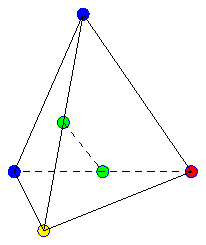
\includegraphics{pics/tetrahedron/tetrahedron1.pdf}
        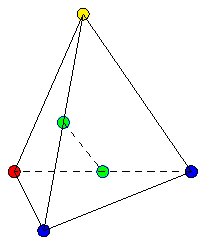
\includegraphics{pics/tetrahedron/tetrahedron2.pdf}
        \caption{Phép quay trục tạo bởi trung điểm hai cạnh đối nhau}
    \end{figure}

    Như hình trên ta thấy nếu chọn trục quay là đường thẳng nối trung điểm 2 cạnh đối diện (2 điểm xanh lá) thì đỉnh trên và đỉnh dưới đổi chỗ cho nhau (xanh và vàng), đỉnh trái và đỉnh phải đổi chỗ cho nhau (xanh và đỏ).

    Ta giải bài này như sau:

    Đầu tiên ta đánh số các đỉnh của tứ diện (như hình)

    \begin{figure}[ht!]
        \centering
        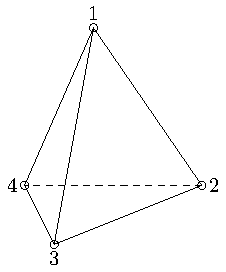
\includegraphics{pics/tetrahedron/tetrahedron3.pdf}
        \caption{Đánh số hình}
    \end{figure}
    
    Ta có 3 trường hợp biến đổi sau:

    \underline{Trường hợp 1}. Giữ nguyên 1 đỉnh và trục quay là đường thẳng đi qua đỉnh đó và tâm của mặt đối diện.

    \begin{figure}[ht!]
        \centering
        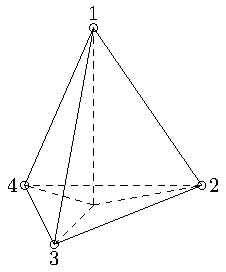
\includegraphics{pics/tetrahedron/tetrahedron4.pdf}
        \caption{Trường hợp 1}
    \end{figure}

    Khi đó phép quay (ngược chiều đồng hồ) tương ứng hoán vị $(1)(2,3,4)$ (quay 60 độ) và $(1)(2,4,3)$ (quay 120 độ).

    Do ta chọn 1 đỉnh cố định thì ta có 4 cách chọn, và với mỗi cách chọn đỉnh cố định ta có thể quay 2 cách nên ta có tổng là 8 hoán vị.

    \underline{Trường hợp 2}. Ta chọn trung điểm 2 cạnh đối nhau và nối lại thành trục quay như hình trong ví dụ. Khi đó tương ứng với hoán vị $(1,4)(2,3)$.

    Ta có $\frac{C^2_4}{2!} = 3$ hoán vị.

    \underline{Trường hợp 3}. Hoán vị đồng nhất $(1)(2)(3)(4)$.

    Tóm lại, tập hợp $M$ ở đây là tập hợp 4 đỉnh của tứ diện, và nhóm tác động lên $M$ là nhóm con 12 phần tử của $\mathcal{S}_4$.

    Như vậy, ví dụ với hoán vị $(1)(2,3,4)$, nếu ta muốn sau phép quay giữ nguyên trạng thái (hay nói cách khác là tìm $M^g$) thì ta
    tô màu đỉnh 1 tùy ý, đỉnh 2-3-4 chung màu (cũng tùy ý).

    Suy ra ta có $3 \cdot 3$ cách tô. Tương tự với các hoán vị dạng $(1,4)(2,3)$.

    Như vậy $t_G = \frac{1}{12}(1 \cdot 3^4 + 8 \cdot 3^2 + 3 \cdot 3^2) = 15$ cách tô màu khác nhau.
\end{example}

Tổng quát, nếu có $k$ màu thì số lớp tương đương là
\[t_G = \frac{1}{12}(1 \cdot k^4 + 8 \cdot k^2 + 3 \cdot k^2) = \frac{1}{12}(k^4 + 11 k^2)\]

\section{Chỉ số chu trình}

Với mỗi hoán vị trong tập $G$ (theo định lý Cayley thì mọi nhóm hữu hạn đều isomorphism với nhóm con nào đó của nhóm hoán vị), ta viết dưới dạng các chu trình độc lập
\[\underbrace{(g_1) (g_2) \ldots (g_{t_{1}})}_{t_1} \underbrace{(g_{j_1} g_{j_2}) (g_{j_3} g_{j_4})\ldots}_{t_2}\]
Nếu ta viết hoán vị dưới dạng các chu trình rời nhau, ta gọi

\begin{tabular}{c c}
    $t_1$ & là số chu trình có độ dài 1 \\
    $t_2$ & là số chu trình có độ dài 2 \\
    $\ldots$ & tương tự \\
    $t_n$ & là số chu trình có độ dài $n$
\end{tabular}

Khi đó, chỉ số chu trình của hoán vị ứng các biến $z_1, z_2, \ldots, z_n$ là
\[I_g (z_1, z_2, ,\ldots, z_n) = z_1^{t_1} z_2^{t_2} \ldots z_n^{t_n}\]

\begin{example}
Xét hoán vị $(1,2,3)(4)(5)(6,7) \in \mathcal{S}_7$

Ta có 2 chu trình độ dài 1, 1 chu trình độ dài 2 và 1 chu trình độ dài 3.
Không có chu trình độ dài 4, 5, 6, 7.

Do đó chỉ số chu trình là 
\[I_g (z_1, z_2, z_3) = z_1^2 z_2^1 z_3^1\]

\end{example}

\begin{remark}
    Bất kì hoán vị nào thuộc $\mathcal{S}_n$ đều thỏa $1 \cdot t_1 + 2 \cdot t_2 + \ldots + n \cdot t_n = n$.
\end{remark}

\begin{definition}{Cyclic index}
    (tạm dịch - \textit{chỉ số chu trình}) của nhóm G là
    \[P_G (z_1, z_2, \ldots, z_n) = \frac{1}{G}\sum_{g \in G} I_g (z_1, z_2, \ldots, z_n)\]
\end{definition}

Nhìn lại ví dụ về tứ diện bên trên, các đỉnh nằm trong cùng chu trình cần được tô cùng màu. Như vậy mỗi $z_i$ tương ứng với một màu.

Từ đó, với ví dụ trên
\[P_G(z_1, z_2, z_3) = \frac{1}{12}\big(z_1^4 + 8 z_1 z_3 + 3 z_2^2\big)\]

Cho mỗi $z_i = 3$ ta có kết quả phép tính theo bổ đề Burnside.

\section{Định lý Polya}

Định lý Polya là một mở rộng cho bổ đề Burnside, cho phép chúng ta đếm số lớp tương đương thỏa mãn điều kiện nhất định (về số lượng phần tử nhất định nhận trạng thái nhất định).

Ví dụ với hình tứ diện như trên nhưng ta thêm điều kiện tô 2 đỉnh màu vàng, 1 đỉnh màu đỏ và 1 đỉnh màu xanh (không tô tổng quát nữa).

Ta ký hiệu tập $R$ là tập hợp các trạng thái có thể nhận của mỗi phần tử $m \in M$.
\[R = \{r_1, r_2, \ldots, r_c \}\]
Ở ví dụ trên thì $R = \{\text{đỏ}, \text{xanh}, \text{vàng}\}$.

Ta thay mỗi $z_i$ trong chỉ số chu trình bằng tổng $\sum_{r \in R} r^i$.

\begin{example}
    Giả sử ta tô màu 4 đỉnh tứ diện với 2 màu $R = \{r_1, r_2\}$.

    Với $z_1$ ta thay bằng $r_1 + r_2$

    Với $z_2$ ta thay bằng $r_1^2 + r_2^2$

    Với $z_3$ ta thay bằng $r_1^3 + r_2^3$

    Khi đó $P_G$ tương đương với
    \[\frac{1}{12}\big[(r_1 + r_2)^4 + 8 \cdot (r_1 + r_2)(r_1^3 + r_2^3) + 3 \cdot (r_1^2 + r_2^2)^2\big]\]
    Khai triển ra (lưu ý là ở đây không có tính giao hoán phép nhân)
    \begin{align*}
        (r_1 + r_2)^4 = & r_1 r_1 r_1 r_1 + r_1 r_1 r_1 r_2 + r_1 r_1 r_2 r_1 + r_1 r_1 r_2 r_2 \\
        + & r_1 r_2 r_1 r_1 + r_1 r_2 r_1 r_2 + r_1 r_2 r_2 r_1 + r_1 r_2 r_2 r_2 \\
        + & r_2 r_1 r_1 r_1 + r_2 r_1 r_1 r_2 + r_2 r_1 r_2 r_1 + r_2 r_1 r_2 r_2 \\
        + & r_2 r_2 r_1 r_1 + r_2 r_2 r_1 r_2 + r_2 r_2 r_2 r_1 + r_2 r_2 r_2 r_2
    \end{align*}

    Mình thấy rằng có 16 cấu hình khác nhau tương ứng 16 cách tô 2 màu cho 4 đỉnh. Tương tự

    \begin{align*}
        (r_1 + r_2) (r_1^3 + r_2^3) & = r_1^4 + r_1 r_2^3 + r_2 r_1^3 + r_2^4 \\
        & = r_1 r_1 r_1 r_1 + r_1 r_2 r_2 r_2 + r_2 r_1 r_1 r_1 + r_2 r_2 r_2 r_2
    \end{align*}

    và cuối cùng

    \begin{align*}
        (r_1^2 + r_2^2)^2 & = r_1^4 + r_1^2 r_2^2 + r_2^2 r_1^2 + r_2^4 \\
        & = r_1 r_1 r_1 r_1 + r_1 r_1 r_2 r_2 + r_2 r_2 r_1 r_1 + r_2 r_2 r_2 r_2
    \end{align*}

    Việc không có tính giao hoán với phép nhân làm biểu thức cồng kềnh và phức tạp.
    Do đó mình thêm một tập hợp $W$ là vành giao hoán, và xét ánh xạ $w: R \mapsto W$ với $w(r_i) = w_i$.

    Khi đó nếu thay $r_i$ bởi $w_i$ vào bên trên biểu thức sẽ rất đẹp
    \[P_G(w_1, w_2) = \frac{1}{12} \big[(w_1 + w_2)^4 + 8 (w_1 + w_2) (w_1^3 + w_2^3) + 3 (w_1^2 + w_2^2)^2\big]\]

    Khai triển và thu gọn ta có
    \begin{align*}
    P_G(w_1, w_2) & = \frac{1}{12} \big[12 w_1^4 + 12 w_1^3 w_2 + 12 w_1^2 w_2^2 + 12 w_1 w_2^3 + 12 w_2^4\big] \\
    & = w_1^4 + w_1^3 w_2 + w_1^2 w_2^2 + w_1 w_2^3 + w_2^4
    \end{align*}

    Ở đây, định lý Polya nói rằng, số mũ của $w_i$ thể hiện số lượng phần tử của tập $M$ nhận giá trị $r_i$,
    và hệ số trước mỗi toán hạng là số lớp tương đương tương ứng với số lượng phần tử của tập $M$ nhận các giá trị $r_i$.

    Nói cách khác:
    \begin{itemize}[noitemsep]
        \item có 1 lớp tương đương mà 4 đỉnh nhận màu $r_1$
        \item có 1 lớp tương đương mà 3 đỉnh nhận màu $r_1$ và 1 đỉnh nhận màu $r_2$
        \item có 1 lớp tương đương mà 2 đỉnh nhận màu $r_1$ và 2 đỉnh nhận màu $r_2$
        \item có 1 lớp tương đương mà 1 đỉnh nhận màu $r_1$ và 3 đỉnh nhận màu $r_2$
        \item cuối cùng là 1 lớp tương đương mà 4 đỉnh nhận màu $r_2$.
    \end{itemize}
\end{example}

Quay lại vấn đề tô 4 đỉnh tứ diện với 3 màu xanh, đỏ, vàng. Tìm số cách tô 2 đỉnh màu vàng, 1 đỉnh màu đỏ và 1 đỉnh màu xanh.

Đặt $w(\text{vàng}) = x$, $w(\text{đỏ}) = y$ và $w(\text{xanh}) = z$

Ta có
\[P_G = \frac{1}{12} \big[(x + y + z)^4 + 8 \cdot (x + y + z) (x^3 + y^3 + z^3) + 3 \cdot (x^2 + y^2 + z^2)^2\big]\]

Như vậy đề bài tương ứng việc tìm hệ số của hạng tử $x^2 yz$ trong biểu thức trên. Mình tính ra kết quả là 1.
\chapter{Ba đường Conic}

Ba đường Conic bao gồm ellipse, hyperbol và parabol.

\section{Ellipse}

\begin{defblock}{Ellipse}

    Đường ellipse là tập hợp các điểm sao cho tổng khoảng cách từ nó tới 2 điểm cố định là 1 hằng số.
\end{defblock}

Nghĩa là, với 2 điểm cố định $F_1, F_2$, tập hợp các điểm $M$ sao cho $M F_1 + M F_2 = 2a$ với $a$ là hằng số tạo thành đường ellipse.

Ở trên hệ tọa độ, nếu ta chọn $F_1$ và $F_2$ nằm trên $Ox$ và đối xứng qua $Oy$, tức là $F_1 = (-c, 0)$ và $F_2 = (c, 0)$, thì các điểm $M = (x, y)$ nằm trên ellipse thỏa

$$MF_1 + MF_2 = \sqrt{(x+c)^2 + y^2} + \sqrt{(x-c)^2 + y^2} = 2a$$

Tương ứng với biển đổi thành phương trình

$$\frac{x^2}{a^2} + \frac{y^2}{a^2 - c^2} = 1$$

Đặt $b^2 = a^2 - c^2$ thì phương trình của ellipse trở thành

$$\frac{x^2}{a^2} + \frac{y^2}{b^2} = 1$$

Phương trình này gọi là \textbf{phương trình chính tắc}.

\begin{figure}[ht]
    \centering
    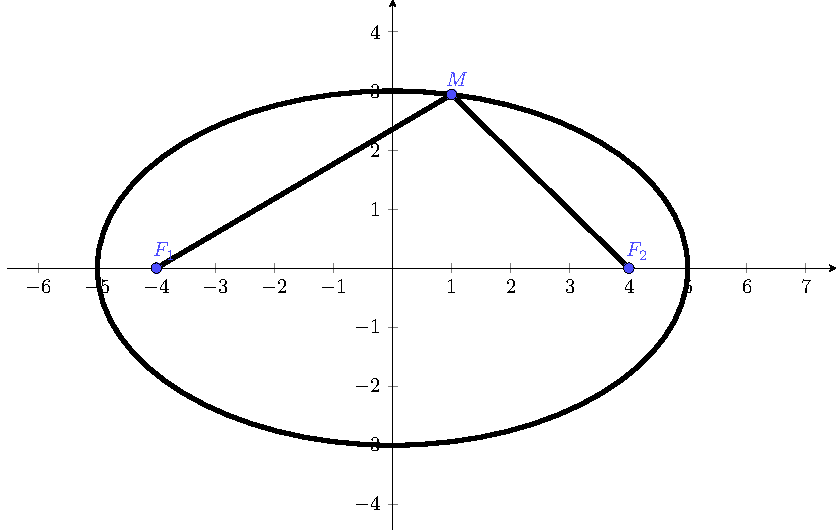
\includegraphics[width=\textwidth]{pics/conics/ellipse.pdf}
    \caption{Ellipse với phương trình $\frac{x^2}{25} + \frac{y^2}{9} = 1$}
\end{figure}

Trong phương trình $$\frac{x^2}{a^2} + \frac{y^2}{b^2} = 1$$

thì $a$ là khoảng cách từ tâm tới 2 biên trái hoặc phải, nên $a$ là \textbf{độ dài bán trục lớn}.

Tương tự, $b$ là \textbf{độ dài bán trục nhỏ} (khoảng cách từ tâm tới 2 biên trên dưới).

Từ cách đặt $b^2 = a^2 - c^2$ tương đương $c^2 = a^2 - b^2$ thì $c$ gọi là \textbf{tiêu cự} của ellipse.

Các điểm $F_1, F_2$ gọi là \textbf{tiêu điểm} của ellipse.

Với ví dụ trên $\frac{x^2}{25} + \frac{y^2}{9} = 1$ thì $a=5, b=3$. Suy ra $c=4$ (lưu ý là $a, b > 0$ và $c \geq 0$).

Các đỉnh nằm ở các tọa độ $(-a, 0), (a, 0), (0, b), (0, -b)$. Các tiêu điểm nằm ở $(-c, 0), (c, 0)$.

\begin{remark}
    Khi $c=0$, tức là 2 tiêu điểm trùng nhau, ta có đường tròn.
\end{remark}

Tâm sai của ellipse là $e = \frac{c}{a} < 1$

\section{Hyperbol}

\begin{defblock}{Hyperbol}

    Đường hyperbol là tập hợp các điểm sao cho giá trị tuyết đối hiệu số khoảng cách từ nó tới 2 điểm cố định là 1 hằng số.
\end{defblock}

Nghĩa là, với 2 điểm cố định $F_1, F_2$, tập hợp các điểm $M$ sao cho $| M F_1 - M F_2 | = 2a$ với $a$ là hằng số tạo thành đường hyperbol.

Ở trên hệ tọa độ, nếu ta chọn $F_1$ và $F_2$ nằm trên $Ox$ và đối xứng qua $Oy$, tức là $F_1 = (-c, 0)$ và $F_2 = (c, 0)$, thì các điểm $M = (x, y)$ nằm trên hyperbol thỏa

$$| MF_1 - MF_2 | = | \sqrt{(x+c)^2 + y^2} - \sqrt{(x-c)^2 + y^2} | = 2a$$

Tương ứng với biển đổi thành phương trình

$$\frac{x^2}{a^2} - \frac{y^2}{a^2 - c^2} = 1$$

Đặt $b^2 = a^2 - c^2$ thì phương trình của hyperbol trở thành

$$\frac{x^2}{a^2} - \frac{y^2}{b^2} = 1$$

Đường hyperbol cắt trục $Ox$ tại 2 điểm $A_1 = (-a, 0)$ và $A_2 = (a, 0)$.

Tiêu điểm của hyperbol ở $F_1 = (-c, 0)$ và $F_2 = (c, 0)$.

Đường hyperbol có 2 tiệm cận là đường thẳng $y = \frac{b}{a} x$ và $y = -\frac{b}{a} x$.

Tâm sai của hyperbol là $e = \frac{c}{a} > 1$.

\section{Parabol}

\begin{defblock}{Parabol}

    Đường parabol là tập hợp các điểm cách đều một điểm cố định và một đường thẳng cố định.

\end{defblock}

\begin{figure}[ht]
    \centering
    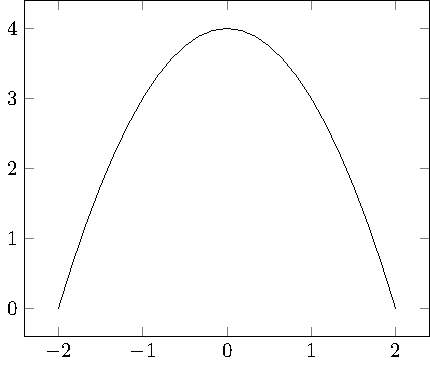
\includegraphics{pics/conics/parabola.pdf}
    \caption{Parabol với phương trình $y = -x^2 + 4$}
\end{figure}

Nghĩa là, với 1 điểm cố định $F$ và đường thẳng cố định $(d)$, parabol là tập hợp các điểm $M$ sao cho $MF = d(M, d)$ với $d(M, d)$ là khoảng cách từ $M$ tới đường thẳng $(d)$.

Phép dời tọa độ cho phép ta dời một hình parabol có đỉnh ở bất kì điểm nào về gốc tọa độ.

Tức là, không mất tính tổng quát, ta chỉ cần xét các parabol dạng $y=ax^2$ là đủ.

Điểm cố định ở trên được gọi là \textbf{tiêu điểm}. Đường thẳng cố định ở trên gọi là \textbf{đường chuẩn}.

Parabol có tính đối xứng nên tiêu điểm nằm trên $Oy$. Đặt tọa độ của nó là $F = (0, f)$.

Đường chuẩn nằm ngang nên ta có parabol là các điểm $M = (x, y)$ sao cho

$MF = \sqrt{x^2 + (y-f)^2}$ và $d(M, d) = y+f$ 
(trường hợp $M$ trùng với đỉnh nên điều kiện của parabol xảy ra tương đương với $M$ cách đều tiêu điểm và đường chuẩn, nghĩa là đường chuẩn có dạng $y=-f$).

Do đó $\sqrt{x^2 + (y-f)^2} = y + f$. Bình phương và biến đổi ta thu gọn được
$$f = \frac{1}{4a}$$

Thường thì ta đặt $p = f$, khi đó phương trình parabol trở thành 
$$x^2 = 4py$$

Đây là dạng chính tắc của parabol với trục đối xứng dọc.

Tâm sai của parabol là $e = \frac{c}{a} = 1$.

\newpage

%$| \mathbb{N} | = | \mathbb{Z} | ?$
%$f: \mathbb{N} \rightarrow \mathbb{Z}$
%$f(n) = n / 2$ nếu $n$ là số chẵn $\geq 0$
%$f(0)=0$, $f(2)=1$, $f(4)=2$
%$f(n) = (-1-n)/2$ nếu $n$ lẻ
%$f(1) = -1$, $f(3) = -2$, $f(5) = -3$
\chapter{Đại số tuyến tính}

\section{Nhắc lại các khái niệm cơ bản}

\begin{defblock}{Hạng của ma trận}
    
    Cho ma trận $\bm{M}_{m \times n}$ có $m$ hàng và $n$ cột. \textbf{Hạng} của ma trận $\bm{M}$ là cấp của ma trận vuông con lớn nhất của $\bm{M}$ có định thức khác 0.

    \textit{Ký hiệu}. Hạng (hay rank) của ma trận $\bm{M}$ ký hiệu là $r = \rank(\bm{M})$

    \end{defblock}

\begin{remark}
    Nếu $r$ là hạng của ma trận $\bm{M}_{m \times n}$ thì $r \leq \min (m, n)$
\end{remark}
\newpage

\part{Lời giải cho bài tập trong một số sách}
\chapter{Abstract Algebra}

Phần này giải các bài tập trong quyển \textbf{Abstract Algebra: Theory and Applications} của Thomas W. Judson (Stephen F. Austin State University)

\section{Groups (chương 3)}

\subsection{Tóm tắt lý thuyết}

Tập hợp $G$ và toán tử 2 ngôi $\star$ trên $G$ tạo thành một nhóm nếu:

\begin{itemize}
    \item Tồn tại phần tử $e \in G$ sao cho với mọi $g \in G$, $e \star g = g \star e = g$. Khi đó $e$ là phần tử đơn vị của $G$.
    \item Với mọi phần tử $g \in G$, tồn tại $g' \in G$ sao cho $g \star g' = g' \star g = e$. Khi đó $g'$ gọi là phần tử nghịch đảo của $g$ trong $G$.
    \item Với mọi $a, b, c \in G$ thì $a \star (b \star c) = (a \star b) \star c$ (tính kết hợp)
\end{itemize}

Nếu có thêm tính chất $a \star b = b \star a$ với mọi $a, b \in G$ thì $G$ gọi là nhóm giao hoán (nhóm Abel).

\subsection{Bài tập}

7. Đặt $S = \RR \backslash \{-1\}$ và định nghĩa toán tử 2 ngôi trên $S$ là $a \star b = a + b + ab$. Chứng minh rằng $(S, \star)$ là nhóm Abel

\begin{proof}
    \begin{itemize}
        \item Giả sử tồn tại phần tử đơn vị $e$, khi đó $e \star s = s \star e = s$ với mọi $s \in S$. Nghĩa là $e + s + es = s + e + se = s$. Vậy $e + se = 0$ mà $s \neq -1$ nên $e = 0$
        \item Với $e = 0$, giả sử với mọi $s \in S$ có nghịch đảo $s'$. Do $s \star s' = s' \star s = e$ nên $s + s' + ss' = s' + s + s's = e = 0$, tức là $s'(1 + s) = -s$. Vậy $s' = \frac{-s}{1 + s}$
        \item Với mọi $a, b, c \in S$, $a \star (b \star c) = a \star (b + c + bc) = a + (b+c+bc) + a (b+c+bc) = a + b + c + ab + bc + ca + abc$ và $(a \star b) \star c = (a + b + ab) \star c = a + b + ab + c + c(a+b+bc) = a + b + c + ab + bc + ca + abc$. Như vậy $a \star (b \star c) = (a \star b) \star c$, tính kết hợp
    \end{itemize}
\end{proof}

39. Gọi $G$ là tập các ma trận $2 \times 2$ với dạng
$$\begin{pmatrix}
    \cos \theta & -\sin \theta \\ \sin \theta & \cos \theta
\end{pmatrix}$$ với $\theta \in \RR$. Chứng minh rằng $G$ là subgroup của $SL_2 (\RR)$
    
\begin{proof}
        Với $\theta_1, \theta_2 \in \RR$, ta có
        
        \begin{align*}
        & \begin{pmatrix}
            \cos \theta_1 & -\sin \theta_1 \\ \sin \theta_1 & \cos \theta_1
        \end{pmatrix} \begin{pmatrix}
            \cos \theta_2 & -\sin \theta_2 \\ \sin \theta_2 & \cos \theta_2
        \end{pmatrix} \\
        = & \begin{pmatrix}
            \cos \theta_1 \cos \theta_2 - \sin \theta_1 \sin \theta_2 & -\cos \theta_1 \sin \theta_2 - \sin \theta_1 \cos \theta_2 \\ 
            \sin \theta_1 \cos \theta_2 + \cos \theta_1 \sin \theta_2 & -\sin \theta_1 \sin \theta_2 + \cos \theta_1 \cos \theta_2
        \end{pmatrix} \\
        = & \begin{pmatrix}
            \cos (\theta_1 + \theta_2) & -\sin (\theta_1 + \theta_2) \\
            \sin (\theta_1 + \theta_2) & \cos (\theta_1 + \theta_2)
        \end{pmatrix}
        \end{align*}
        
        Suy ra định thức của tích 2 ma trận là

        \begin{align*}
            \det \Biggl(\begin{pmatrix}
                \cos (\theta_1 + \theta_2) & -\sin (\theta_1 + \theta_2) \\
                \sin (\theta_1 + \theta_2) & \cos (\theta_1 + \theta_2)
            \end{pmatrix}\Biggr)
            = & 1 \cdot 1 = 1
        \end{align*}
        Như vậy phép nhân 2 ma trận có dạng trên đóng trên $SL_2 (\RR)$.
        
        Phần tử đơn vị là $\begin{pmatrix}
        1 & 0 \\ 0 & 1
        \end{pmatrix}$ tương ứng với $\theta = 0$
        
        Phần tử nghịch đảo là $\begin{pmatrix}
        \cos (-\theta) & -\sin (-\theta) \\ \sin (-\theta) & \cos (-\theta)
        \end{pmatrix}$ suy ra từ công thức định thức ban nãy
        
        Cuối cùng, phép nhân ma trận có tính kết hợp. Như vậy $G$ là subgroup của $SL_2 (\RR)$
        
\end{proof}

47. Đặt $G$ là nhóm và $g \in G$. Chứng minh rằng $$Z(G) = \{ x \in G: gx = xg \; \forall \; g \in G \}$$ là subgroup của $G$. Subgroup này gọi là \textbf{center} của $G$

\begin{proof}
    Giả sử trong $G$ có 2 phần tử là $x_1$ và $x_2$ thuộc $Z(G)$. Khi đó

        $x_1 g = g x_1$ và $x_2 g = g x_2$ với mọi $g \in G$.

    Xét phần tử $x_1 x_2$, ta có
    $$(x_1 x_2) g = x_1 (x_2 g) = x_1 (g x_2) = (g x_1) x_2 = g (x_1 x_2)$$ với mọi $g \in G$. Do đó $x_1 x_2 \in Z(G)$ nên $Z(G)$ là subgroup.

\end{proof}

49. Cho ví dụ về nhóm vô hạn mà mọi nhóm con không tầm thường của nó đều vô hạn

Ví dụ tập $\ZZ$ và phép cộng số nguyên. Khi đó mọi nhóm con của $\ZZ$ có dạng $n\ZZ$ với $n \in \ZZ$. Ví dụ

$2\ZZ = \{\cdots, -4, -2, 0, 2, 4, \cdots\}$ với phần tử sinh là $2$

$n\ZZ = \{\cdots, -2n, -n, 0, n, 2n, \cdots\}$ với phần tử sinh là $n$

54. Cho $H$ là subgroup của $G$ và $$C(H) = \{g \in G: gh = hg \; \forall \; h \in H\}$$

Chứng minh rằng $C(H)$ là subgroup của $G$. Subgroup này được gọi là \textbf{centralizer} của $H$ trong $G$

\begin{proof}
    Gọi $g_1$ và $g_2$ thuộc $C(H)$. Khi đó

    $g_1 h = h g_1$ và $g_2 h = h g_2$ với mọi $h \in H$

    Xét phần tử $g_1 g_2$, với mọi $h \in H$ ta có
    $$(g_1 g_2) h = g_1 (g_2 h) = g_1 (h g_2) = (g_1 h) g_2 = (h g_1) g_2 = h (g_1 g_2)$$

    Như vậy $g_1 g_2 \in C(H)$, từ đó $C(H)$ là subgroup của $G$


\end{proof}

\subsection{Kết luận}

Bài tập số 47 và 54 là 2 khái niệm quan trọng cho bổ đề Burnside và định lý Polya.

\section*{Permutation Groups}

\subsection*{Tóm tắt lý thuyết}

Đặt $S_n$ là nhóm hoán vị trên tập $n$ phần tử. Như vậy $S_n$ có $n!$ phần tử.

Mỗi phần tử trong $S_n$ có thể biểu diễn dưới dạng các chu trình (cycle) độc lập (disjoint).

\subsection*{Bài tập}

13. Đặt $\sigma = \sigma_1 \cdots \sigma_m \in S_n$ là tích của các cycle độc lập. Chứng minh rằng order của $\sigma$ là LCM của độ dài các cycle $\sigma_1, \cdots, \sigma_m$.

\begin{proof}
    Đặt $l_i$ là độ dài cycle $\sigma_i$ ($i = 1, \cdots m$). Khi đó $\sigma_i^{k_i l_i}$ sẽ ở dạng các cycle độ dài 1 ($k_i \in \ZZ$).

    Từ đó, $\sigma^l = \sigma_1^l \cdots \sigma_m^l = (1)\cdots(n)$ nếu $l = k_1 l_1 = \cdots k_m l_m$. Số $l$ nhỏ nhất thỏa mãn điều kiện này là $\lcm(l_1, \cdots, l_m)$ (đpcm)

\end{proof}

23. Nếu $\sigma$ là chu trình với độ dài lẻ, chứng minh rằng $\sigma^2$ cũng là chu trình
\begin{proof}
    Giả sử $\sigma = (g_1, g_2, \cdots, g_{n-1}, g_n)$ với $n$ lẻ. Khi đó $\sigma^2 = (g_1, g_3, \cdots, g_n, g_2, g_4, \cdots, g_{n-1})$ cũng là chu trình.
\end{proof}

30. Cho $\tau = (a_1, a_2, \cdots, a_k)$ là chu trình độ dài $k$.

\begin{enumerate}
    \item[(a)] Chứng minh rằng với mọi hoán vị $\sigma$ thì $$\sigma \tau \sigma^{-1} = (\sigma(a_1), \sigma(a_2), \cdots, \sigma(a_k))$$ là chu trình độ dài $k$.
    \item[(b)] Gọi $\mu$ là chu trình độ dài $k$. Chứng minh rằng tồn tại hoán vị $\sigma$ sao cho $\sigma \tau \sigma^{-1} = \mu$
\end{enumerate}

\begin{proof}
    \begin{enumerate}
        \item [(a)] Ta thấy rằng bất kì phần tử nào khác $a_1, a_2, \cdots, a_k$ thì khi qua $\tau$ không đổi, do đó khi đi qua $\sigma \tau \sigma^{-1}$ thì chỉ đi qua $\sigma \sigma^{-1}$ và cũng không đổi. Nói cách khác các phần tử $a_1, a_2, \cdots, a_k$ vẫn nằm trong chu trình nên ta có đpcm.
        \item [(b)] Từ câu (a), với $\mu = (b_1, b_2, \cdots, b_k)$ thì ta chọn $\sigma$ sao cho $b_i = \sigma(a_i)$.
    \end{enumerate}    
\end{proof}


\subsection*{Kết luận}

Bổ đề Burnside và định lý Polya dùng để đếm số cấu hình khác nhau dựa trên nhóm hoán vị.
\section{Cosets (chương 6)}

11. Gọi $H$ là subgroup của nhóm $G$ và giả sử $g_1, g_2 \in G$. Chứng minh các mệnh đề sau là tương đương:

\begin{itemize}
    \item[(a)] $g_1 H = g_2 H$
    \item[(b)] $H g_1^{-1} = H g_2^{-1}$
    \item[(c)] $g_1 H \subseteq g_2 H$
    \item[(d)] $g_2 \in g_1 H$
    \item[(e)] $g_1^{-1} g_2 \in H$ 
\end{itemize}

\begin{proof}
    Từ (a) ra (b): Ta đã biết các coset là rời nhau hoặc trùng nhau, do đó với mọi $g_1 h \in g_1 H$, tồn tại $g_2 h' \in g_2 H$ mà $g_1 h = g_2 h'$. Suy ra $(g_1 h)^{-1} = (g_2 h')^{-1}$ hay $h^{-1} g_1^{-1} = h'^{_1} g_2^{-1}$ (đpcm)

    Từ (a) ra (c): Hiển nhiên

    Từ (a) ra (d): Với mọi $g_1 h \in g_1 H$, tồn tại $g_2 h' \in g_2 H$ sao cho $g_1 h = g_2 h'$, hay $g_2 = g_1 h h'^{-1}$, đặt $h'' = h h'^{-1}$ thì $h'' \in H$ ($H$ là nhóm con) nên $g_1 h'' \in g_1 H$. Suy ra $g_2 \in g_1 H$

    Từ (a) ra (e): Tương tự, ta có $g_1 h = g_2 h'$, suy ra $h h'^{-1}= g_1^{-1} g_2 \in H$

\end{proof}


16. Nếu $g h g^{-1} \in H$ với mọi $g \in G$ và $h \in H$, chứng minh rằng right coset trùng với left coset

\begin{proof}
    Do $g h g^{-1} \in H$ nên tồn tại $h' \in H$ sao cho $g h g^{-1} = h'$. Tương đương $g h = h' g$ với mọi $h \in H$ nên $g H = H g$. Điều này đúng với mọi $g \in G$ nên các right coset trùng left coset.
\end{proof}

17. Giả sử $[G:H]=2$. Chứng minh rằng nếu $a, b$ không thuộc $H$ thì $ab \in H$.

\begin{proof}
    Ta biết rằng 2 coset ứng với 2 phần tử $g_1, g_2$ bất kì là trùng nhau hoặc rời nhau.

    Do đó với $eH = H$, ta suy ra 2 coset của $G$ là $H$ và $G \backslash H$.

    Vì $a, b \not\in H$ nên coset của chúng trùng nhau. Và nghịch đảo của $a$ cũng nằm trong $G \backslash H$ vì nếu nghịch đảo của $a$ nằm trong $H$ thì $a$ cũng phải nằm trong $H$.

    Suy ra $a^{-1} H = b H$. Nghĩa là tồn tại 2 phần tử $h_1, h_2 \in H$ sao cho $a^{-1} h_1 = b h_2$, tương đương $h_1 h_2^{-1} = a b \in H$ (đpcm).
\end{proof}

21. Gọi $G$ là cyclic group với order $n$. Chứng minh rằng có đúng $\phi(n)$ phần tử sinh của $G$

\begin{proof}
    Gọi $g$ là một phần tử sinh của $G$. Khi đó $g$ sinh ra tất cả phần tử trong $G$, hay nói cách khác các phần tử trong $G$ có dạng $g^i$ với $0 \leq i < n$.

    Như vậy một phần tử $h = g^i$ cũng là phần tử sinh của $G$ khi và chỉ khi $\gcd(i, n) = 1$ và có $\phi(n)$ số $i$ như vậy (đpcm).

\end{proof}
\section{Isomorphism (chương 9)}

\subsection{Tóm tắt lý thuyết}

Cho 2 nhóm $(G, \star)$ và $(H, *)$. Ánh xạ $\varphi: G \rightarrow H$ được gọi là isomorphism từ $G$ tới $H$ nếu:

\begin{itemize}
    \item với mọi $g_1, g_2 \in G$ thì $\varphi(g_1 \star g_2) = \varphi(g_1) * \varphi(g_2)$
    \item $\varphi$ là song ánh (one-to-one và onto)
\end{itemize}

\subsection{Bài tập}

18. Chứng minh rằng subgroup của $\QQ^*$ gồm các phần tử có dạng $2^m 3^n$ với $m, n \in \ZZ$ là internal direct product tới $\ZZ \times \ZZ$

\begin{proof}
    Xét ánh xạ $\varphi: \QQ^* \rightarrow \ZZ \times \ZZ$, $\varphi(2^m 3^n) = (m, n)$

    Hàm này là well-defined vì với $m$ cố định thì mỗi phần tử $2^m 3^n$ chỉ cho ra một phần tử $(m, n)$. Tương tự với cố định $n$.

    Hàm này là đơn ánh (one-to-one) vì với $m_1 = m_2$ và $n_1 = n_2$ thì $2^{m_1} 3^{n_1} = 2^{m_2} 3^{n_2}$.

    Hàm này cũng là toàn ánh vì với mỗi cặp $(m, n)$ ta đều tính được $2^m 3^n$.

    Vậy hàm $\varphi$ là song ánh.

    Thêm nữa, 
    \begin{align*}
        \varphi(2^{m_1} 3^{n_1} \cdot 2^{m_2} 3^{n_2})& = \varphi(2^{m_1 + m_2} 3^{n_1 + n_2}) \\
        & = (m_1 + m_2, n_1 + n_2) = (m_1, n_1) + (m_2, n_2) \\
        & = \varphi(2^{m_1} 3^{n_1}) \varphi(2^{m_2} 3^{n_2})
    \end{align*}

    Vậy $\varphi$ là homomorphism, và là song ánh nên là isomorphism.

    \end{proof}

20. Chứng minh hoặc bác bỏ: mọi nhóm Abel có order chia hết bởi 3 chứa một subgroup có order là 3

\begin{proof}
    Gọi order của nhóm Abel là $n=3k$, và $g$ là phần tử sinh của nhóm Abel đó. Như vậy $g^n = g^{3k} = e$.

    Nếu ta chọn $h = g^k$ thì $h^3 = e$, khi đó subgroup được sinh bởi $h$ có order 3 (đpcm).
\end{proof}

21. Chứng minh hoặc bác bỏ: mọi nhóm không phải Abel có order chia hết bởi 6 chứa một subgroup có order 6

\begin{proof}
    Với $\mathcal{S}_3$ có order là 6 nhưng không có nhóm con nào order 6 (nhóm con chỉ có order 1, 2 hoặc 3) (bác bỏ).
\end{proof}

22. Gọi $G$ là group với order 20. Nếu $G$ có các subgroup $H$ và $K$ với order 4 và 5 mà $hk=kh$ với mọi $h \in H$ và $k \in K$, chứng minh rằng $G$ là internal direct product của $H$ và $K$

\begin{proof}
    Ta chứng minh $H \cap K = \{ e \}$. Giả sử tồn tại phần tử $m \in H \cap K$, khi đó do $m \in H$ nên $mk = km$ với mọi $k \in K$. Tuy nhiên $m \in K$ do đó điều này xảy ra khi và chỉ khi $m = e$.

    Như vậy $H \cap K = \{ e \}$.
\end{proof}

\subsection{Kết luận}

Isomorphism cho phép chúng ta chuyển từ việc tính toán trên một nhóm này thành tính toán trên nhóm khác dễ hơn (về mặt số học, toán tử).

\begin{theorem}[Định lý Cayley]
    Mọi nhóm hữu hạn $n$ phần tử isomorphism với nhóm con nào đó của nhóm hoán vị $S_n$
\end{theorem}

\part{Lịch sử toán học}
Trong lịch sử, từ xa xưa con người đã biết tính toán, sử dụng chúng cho công việc hằng ngày.

Chúng ta không biết ai là người đầu tiên phát minh ra lịch, cũng như cách tính toán để phân chia ruộng đất, tài sản trong các nền văn minh cổ.
Những điều đó được đúc kết theo kinh nghiệm qua hàng chục, thậm chí hàng trăm năm tri thức con người.

Cho tới khi những nhân vật sau (và nhiều nhân vật tương tự khác) đi du lịch Ai Cập và phương đông (ý mình là đi du học).

Đầu tiên phải nhắc tới Euclid, người đã quá quen thuộc với học sinh phổ thông với tiên đề Euclid. Hệ tiên đề Euclid đề ra trở thành cơ sở cho hình học. Bộ sách \textit{Elements} của ông được cho là bộ sách giáo khoa đầu tiên trên thế giới và những gì ghi trong đó khá giống với những gì được giảng dạy ở trường học chúng ta ngày nay.

Nhưng ông đã không lường trước được 1 điều: thế hệ sau đã "thêm mắm dặm muối" và biến đổi hình học của ông thành hình học Phi-Euclid. Từ đó mở ra những khả năng lớn hơn của toán học.

Pythagoras: định lý Pythagoras trong tam giác vuông có lẽ là định lý đầu tiên mà học sinh tiếp cận. Phát biểu rất đơn giản:

\begin{theorem}[Định lý Pythagoras]
    Trong tam giác vuông, bình phương cạnh huyền bằng tổng bình phương hai cạnh góc vuông.

    Nói cách khác, tam giác có 2 cạnh góc vuông lần lượt là $a$ và $b$, cạnh huyền độ dài là $c$ thì
    \[a^2 + b^2 = c^2\]
\end{theorem}

Thật ra trước thời Pythagoras rất lâu, người Ai Cập đã biết tới phương pháp này. Có nhiều bằng chứng về các cuộn giấy papyrus ghi lại các bộ số nguyên $(a, b, c)$ mà $a^2 + b^2 = c^2$ được tìm thấy khi khai quật.

Tuy nhiên thời đó con người chỉ làm việc với các số nguyên, chính xác hơn là các số tự nhiên vì chúng "tự nhiên" xuất hiện trong đời sống.

Pythagoras là người đầu tiên nhắc tới \textbf{proof} (chứng minh) trong toán học. Một phát biểu, định lý chỉ đúng khi có một chứng minh đúng đắn cho nó. Các bước suy luận trong chứng minh dựa trên một hệ tiên đề (axiom) cho trước.
Các tiên đề này hiển nhiên đúng, từ đó các suy luận chính xác sẽ cho kết quả chính xác.

Cho tới khi Fermat phán:

\begin{theorem}[Định lý cuối cùng của Fermat]
    Không tồn tại một cách phân tích tam thừa thành tổng 2 tam thừa, tứ thừa thành tổng 2 tứ thừa, hay tổng quát hơn

    Với mọi số nguyên $n \geq 3$, không tồn tại bộ số nguyên $(a, b, c)$ sao cho
    \[a^n + b^n = c^n\]
\end{theorem}

Và cú lừa có lẽ là lớn nhất thời đại: \textit{"Tôi đã tìm được chứng minh cho mệnh đề kỳ diệu này nhưng lề sách quá chật không thể viết được"}.

Vâng, cái chứng minh kỳ diệu mà ông nói đã khiến các nhà toán học thiên tài bế tắc trong suốt hơn 300 năm, sử dụng nhiều công cụ phức tạp không có ở thời Fermat và hoàn thiện bởi bài báo 200 trang của Andrew Wiles.

Nghĩa là 200 lề sách cũng không viết đủ chứng minh cho định lý cuối cùng của Fermat!!!

Phần này mình làm vì đam mê tìm hiểu lịch sử toán. Ở đây ghi lại cuộc đời và công trình của các nhà toán học lớn trên thế giới suốt chiều dài lịch sử.

Phần này lấy cảm hứng từ quyển \textit{Thiên tài và số phận} và \textit{Định lý cuối cùng của Fermat} của thầy Lê Quang Ánh, thông tin tham khảo dựa trên nhiều nguồn (chủ yếu là quyển \textit{Men of Mathematics} của E.T.Bell).

Tuy nhiên thông tin về cuộc đời của các nhà toán học đã có khá nhiều, mình sẽ trình bày theo cách hiểu của bản thân và đôi khi tập trung nhiều vào các công trình mức cơ sở.

Ngoại trừ phần lịch sử của nhà toán học, mình sẽ trình bày các định lý, khái niệm, ứng dụng của họ theo cách viết, cách trình bày của toán học hiện đại ngày nay để dễ tiếp cận.

\chapter{Euclid}

Lúc mình học cấp 2, tiên đề Euclid được học là một trong 5 tiên đề hình học của Euclid. Nội dung tiên đề đó như sau:

\begin{axiom}[Tiên đề Euclid]
    Qua một điểm nằm ngoài đường thẳng cho trước, ta vẽ được một và chỉ một đường thẳng song song với đường thẳng đã cho.
\end{axiom}

Trong hình học Euclid, hình được vẽ trên \textit{mặt phẳng}. Ở đó, với 2 điểm phân biệt ta vẽ được duy nhất một đường thẳng đi qua 2 điểm đó.

Nếu chúng ta chỉ lấy phần ở giữa 2 điểm, ta có \textit{đoạn thẳng}. Nếu ta lấy phần ở ngoài 2 điểm nhưng chỉ một phía (đường thẳng kéo dài 2 phía) ta có nửa đường thẳng (hay còn gọi là tia).

Chúng ta có 2 công cụ để vẽ hình: thước và compa. Từ 2 công cụ này ta có thể vẽ được rất nhiều hình dạng như chia đôi góc (phân giác), chia đôi cạnh (lấy trung điểm), vẽ đường tròn, đường thẳng.

Tuy nhiên chúng lại có giới hạn: không thể chia 3 góc, hay không thể vẽ được hình đa giác đều 7 cạnh.

Những bài toán nhìn có vẻ đơn giản nhưng phải tới nhiều thế hệ sau, con người mới tìm được cách chứng minh rằng một hình nào đó có dựng được bằng thước và compa hay không.

Tiên đề là những mệnh đề mà ta thừa nhận tính đúng đắn của nó không cần chứng minh. Tuy nhiên sự đúng đắn phải được kiểm nghiệm từ thực tiễn.
Cơ sở của hình học Euclid gồm hệ các tiên đề làm nền móng cho các chứng minh toán học về sau.
\chapter{Zeno}

Zeno là nhà triết học nổi tiếng của Hy Lạp. Trong toán học, ông nổi tiếng về nghịch lý Zeno:

Archiles chạy đua với rùa. Do Archiles chạy nhanh hơn nên sẽ chấp rùa chạy trước. Khi đó Zeno bảo rằng Archiles sẽ không thể đuổi kịp rùa.

Phát biểu nghe rất mâu thuẫn nhưng được Zeno lý giải như sau:

\begin{itemize}[noitemsep]
    \item Giả sử ban đầu Archiles xuất phát sau con rùa một khoảng $d_1$
    \item Archiles mất một khoảng thời gian $t_1$ để đi hết quãng đường $d_1$ đó. Tuy nhiên trong khoảng thời gian $t_1$ đó con rùa cũng đi được một quãng đường $d_2$
    \item Archiles lại mất thêm một khoảng thời gian $t_2$ để đi hết quãng đường $d_2$. Nhưng rùa cũng đã đi được một đoạn $d_3$ nào đó trong thời gian $t_2$ rồi.
    \item Và cứ tiếp tục như thế, ta thấy rằng khoảng cách $d_n$ giữa 2 người sẽ nhỏ dần đi, nhưng không bao giờ chạm 0. Nói cách khác Archiles không thể bắt kịp con rùa.
\end{itemize}

Có gì đó rất \textit{không ổn} ở đây. Rõ ràng trên thực tế Archiles chắc chắn sẽ bắt kịp con rùa trong một khoảng thời gian nhất định. Nhưng tại sao suy luận của Zeno lại cho ra kết quả lạ thường vậy?

Câu trả lời là ở \textbf{vô cực}. Nói theo toán học hiện đại, khoảng cách $d_n$ tiến về 0 khi $n$ tiến ra vô cùng.

Tuy nhiên sự vô cùng chưa được hiểu đúng ở thời của Zeno. Việc này sẽ được giải quyết ở thời của Cantor.
\chapter{Cauchy}

\begin{theorem}[Bất đẳng thức AM-GM]
    Với 2 số không âm $a, b$, ta luôn có
    \[a+b \geq 2 \sqrt{ab}\]
    Dấu bằng xảy ra khi $a = b$.
\end{theorem}

Tổng quát cho $n$ số ta có

\begin{theorem}[Bất đẳng thức AM-GM tổng quát]
    Với $n$ số không âm $a_1, a_2, \ldots, a_n$, ta luôn có
    \[a_1 + a_2 + \ldots + a_n \geq n \sqrt[n]{a_1 a_2 \ldots a_n}\]
    Dấu bằng xảy ra khi $a_1 = a_2 = \ldots = a_n$.
\end{theorem}

Thực tế, bất đẳng thức Cauchy (còn gọi là bất đẳng thức Cauchy-Schwarz) có thể hiểu theo cách cơ bản như sau:

\begin{theorem}[Cauchy-Schwarz]
    Với 2 bộ số $(a_1, a_2, \ldots, a_n)$ và $(b_1, b_2, \ldots, b_n)$ ta có
    \[(a_1^2 + a_2^2 + \ldots + a_n^2) (b_1^2 + b_2^2 + \ldots + b_n^2) \geq (a_1 b_1 + a_2 b_2 + \ldots + a_n b_n)^2\]

    Dấu bằng xảy ra khi $\frac{a_1}{b_1} = \frac{a_2}{b_2} = \ldots = \frac{a_n}{b_n}$
\end{theorem}

Theo ngôn ngữ đại số tuyến tính thì định lý Cauchy-Schwarz như sau:

\begin{theorem}[Cauchy-Schwarz]
    Trong không gian Euclid, với mọi vector $\vec{x}$ và $\vec{y}$ thì 
    \[\lVert \vec{x} \rVert \cdot \lVert \vec{y} \rVert \geq \langle \vec{x}, \vec{y} \rangle\]
    
    Có nghĩa là, tích độ dài 2 vector bất kì lớn hơn hoặc bằng tích vô hướng của chúng.

    Dấu bằng xảy ra khi 2 vector đó cùng phương.
\end{theorem}
\chapter{Nicolai Ivanovich Lobachevsky}

Nhà toán học vĩ đại người Nga 
\begin{otherlanguage}{russian}
    Лобачевский Николай Иванович   
\end{otherlanguage}
(N.I. Lobachevsky) (1792-1856) là người có công rất lớn trong việc xây dựng hình học phi Euclid.




\end{document}